\documentclass{article}

% if you need to pass options to natbib, use, e.g.:
% \PassOptionsToPackage{numbers, compress}{natbib}
% before loading nips_2017
%
% to avoid loading the natbib package, add option nonatbib:
% \usepackage[nonatbib]{nips_2017}
\PassOptionsToPackage{numbers, compress}{natbib}
\usepackage[final]{nips_2017}

% to compile a camera-ready version, add the [final] option, e.g.:
% \usepackage[final]{nips_2017}

\usepackage[utf8]{inputenc} % allow utf-8 input
\usepackage[T1]{fontenc}    % use 8-bit T1 fonts
\usepackage{hyperref}       % hyperlinks
\usepackage{url}            % simple URL typesetting
\usepackage{booktabs}       % professional-quality tables
\usepackage{amsfonts}       % blackboard math symbols
\usepackage{nicefrac}       % compact symbols for 1/2, etc.
\usepackage{microtype}      % microtypography
\usepackage{graphicx}
\usepackage{amsmath}
\graphicspath{{graphics/}}

\title{Using Molecules for Machine-Learning Chemistry via MoleculeNet}

% The \author macro works with any number of authors. There are two
% commands used to separate the names and addresses of multiple
% authors: \And and \AND.
%
% Using \And between authors leaves it to LaTeX to determine where to
% break the lines. Using \AND forces a line break at that point. So,
% if LaTeX puts 3 of 4 authors names on the first line, and the last
% on the second line, try using \AND instead of \And before the third
% author name.

\author{
  Adarsh Dave \\
  \texttt{ardave} \\
  \And
  Jake Parker \\
  \texttt{jlparker}
  \And
  Sarah Malle \\
  \texttt{smallepa}
  %% examples of more authors
  %% \And
  %% Coauthor \\
  %% Affiliation \\
  %% Address \\
  %% \texttt{email} \\
  %% \AND
  %% Coauthor \\
  %% Affiliation \\
  %% Address \\
  %% \texttt{email} \\
  %% \And
  %% Coauthor \\
  %% Affiliation \\
  %% Address \\
  %% \texttt{email} \\
  %% \And
  %% Coauthor \\
  %% Affiliation \\
  %% Address \\
  %% \texttt{email} \\
}

\begin{document}
% \nipsfinalcopy is no longer used

\maketitle

\section{Introduction and Related Work}
Key technology problems in pharmacology, renewable energy, and agriculture could be solved with novel, high-performance materials and chemical compounds. Breakthroughs via physical experiment are often slow-to-arrive, leading to many researchers harnessing high-performance computing for so-called "rational materials design" via  high-throughput simulation and "virtual screening" [1]. The corresponding increase in data availability has lead to a surge of machine-learning research.

The core task of rational materials design is predicting chemical and materials properties from first principles, i.e. by solving the mathematics of chemical physics / quantum mechanics using only chemical compounds as inputs, without relying on empirical data. Thus, a corresponding goal for machine-learning techniques is to predict material properties using only the chemical compounds as input. Another motivation for training models on only molecules is that molecule geometry represent the largest, most centralized and most standardized data-sets in chemical informatics - with 94 million compounds in PubChem alone.

However, molecular-level machine-learning presents tricky issues. First, there is the limited availability of "ground-truth" experiment label data and  such data is also scattered and heterogeneous in format, much of it stuck in PDF tables in scientific papers. Second, scientists often want to predict many labels at different scales, e.g. electronic structure properties up to physiological impacts. Third, molecules themselves are variable in dimension, connectivity, and conformers. [2].

Past work on the subject reflects these challenges. For example, Tetko et al. predicted melting points for drug-like compounds with numerous machine-learning frameworks; however, the best results there (from an associative neural network) still resulted in an RMSE of ~30 degrees C, over a data-set of 50,000 molecules[3]. Such errors make the model nearly useless for any interested materials scientist.

Any attempt to utilize molecule geometries in a machine-learning model faces two key choices: 1) choice of featurization and 2) choice of machine-learning framework. Much work has been published about molecule representation, and it remains a hotly-debated academic field. MoleculeNet, presented by the Pande lab at Stanford last year, is a new benchmark for making these two choices using molecular inputs. Our goal is to understand and replicate their results [2].

Our main task is to recreate the paper's benchmark cases with physical chemistry and quantum mechanical data-sets - these results can be seen in Figs 12, 14, and 15 and Table 3 in Reference 2. Because our team is primarily interested in physical chemistry and quantum mechanics (as opposed to physiology and biophysics), we've chosen this smaller data-set.

By replicating the Pande group's work, we hope to gain insight into how a data-scientist might approach featurizing molecules, as well as choice of model. Additional concerns such as splitting up heterogeneous data into training, testing, and validation sets, as well as hyper-parameter optimization, will be addressed in this project.

After recreating these benchmarks, we will focus on how additional data (particularly systematically erroneous data that is of significantly higher availability than experimental data) might improve such models.

In this progress report, we will cover below is a list of topics from MoleculeNet that we will cover:
\begin{enumerate}
\item Data-set description and splitting
\item Featurization: ECFP, Coulomb Matrix
\item Modeling: Random Forest
\item Parameter tuning: Hyperparameter optimization [4]

\end{enumerate}

\section{Data-set}

The first data analyzed was John Delaney's ESOL dataset [5]. ESOL gives SMILES representations of molecules (a unique string representation of the atomic components of the molecule), and their log solubilities in water. There is a long history of predicting solubility via so-called quantitative-structure-property-relationships (QSPR) models in chemistry (a forerunner of modern machine-learning chemical informatics). Benchmark values for test-set mean-absolute-error in predicting solubility from this data-set range from 0.40 to 0.70 in log-solubility. A histogram of the data is shown below:

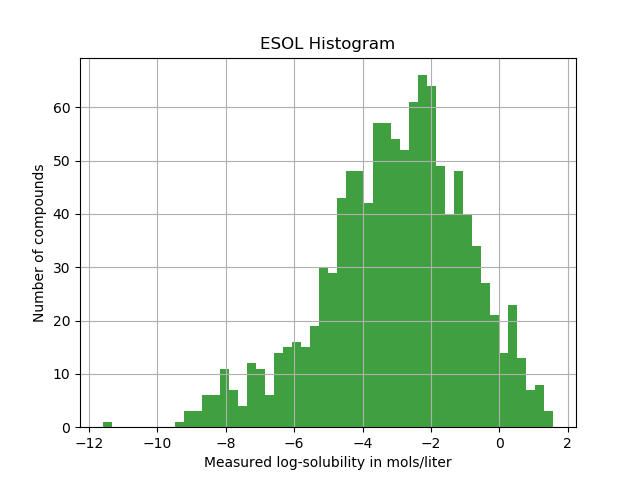
\includegraphics[width=0.75\textwidth]{esolhist}

\section{Methods}

We utilize DeepChem - a Python library built atop TensorFlow by authors of References 2 and 3 - supplemented by scikit-learn for the core machine-learning models, and RDkit for general molecule representation and transformation. In particular for this report, RDkit was used to transform from SMILES representation of molecules to 3D geometries.

\subsection{Featurization}

As of this report, we've looked at two standard, widely-used featurization methods for representing molecules to machine-learning models.

\subsubsection{Extended Connectivity Fingerprint}

ECFP maps a molecule out in concentric circles [6]. It captures properties like atomic number, number of non-hydrogen neighbors, ring structures, etc.. These properties are captured in a fixed-length bit string via a hashing process. It takes two main parameters to generate the features: 1) the length of the bit string (we use 1024 as in prior literature), and 2) the diameter of the circular neighborhoods, for which we use 6 (again as in prior literature).

\subsubsection{Coulomb Matrix}

The Coulomb matrix is a physics-inspired representation of the molecule as a network. Atoms are nodes and edges are weighted as the pair-wise energetic interaction. Off-diagonal elements correspond to the Coulomb repulsion between atoms I and J, while diagonal elements encode a polynomial fit of atomic energies to nuclear charge [7].
  \begin{equation}
    C_{ij}=
    \begin{cases}
      0.5 Z_i^{2.4}, & \text{if}\ i=j \\
      \frac{Z_i Z_j}{|R_i - R_j|}, & \text{otherwise}
    \end{cases}
  \end{equation}
 
\subsection{Splitting of Data-sets}

Molecules vary widely across compound classes, but are fairly similar within a given class (e.g. alkanes, linear carbonates...). A good prediction model would be able to accurately predict on class A of molecules, even if it was trained on class B of molecules. To ensure scoring of this type, we use scaffold splitting based on Bemis Murcko clustering to ensure that different classes of molecules are kept within a set, whether that is training, validation, or testing set. 

Essentially, Bemis Murcko cares only about 2D structure of the molecule (not atom type, hybridization, or bond order). The original developers of the clustering algorithm found that, in a 6000 drug data-set, there were 1200 visible structural categories, but that half the data came from only 32 structural categories [8].

Thus, all molecules that share an underlying 2D scaffold are placed into the same split, ensuring that each split contains dissimilar molecules.

We also compared scaffold split to a random split.

\subsection{Transformation}

This project concerns regression data-sets with continuous labels. Thus, we transformed our data-sets to have zero-mean and unit standard deviation.

\subsection{Models}

\subsubsection{Random Forest Regressor}

The random forest is similar to the boosted decision trees we covered in lecture, in that many trees are fit to sub-samples of the data-set and averaged. The two hyper-parameters used in this model: the number of estimators/trees, and the maximum number of features considered at each split in relation to the number of estimators.

\subsubsection{Hyperparameter Optimization}

The validation set was used to optimize hyperparameters. We generally used a grid search test of hyperparameters, testing each combination to maximize some accuracy metric on the validation set.

\section{Preliminary Results}

We fit a number of random forests to the ESOL data-set to assess prediction accuracy. The first set split the data-set via Bemis Burcko scaffold, and optimized hyper-parameters to 100 estimators, maximum features as sqrt(100)=10. This resulsted in a 2.5 RMSE, larger than the MoleculeNet benchmark of approximately 1.5 RMSE for random forests.

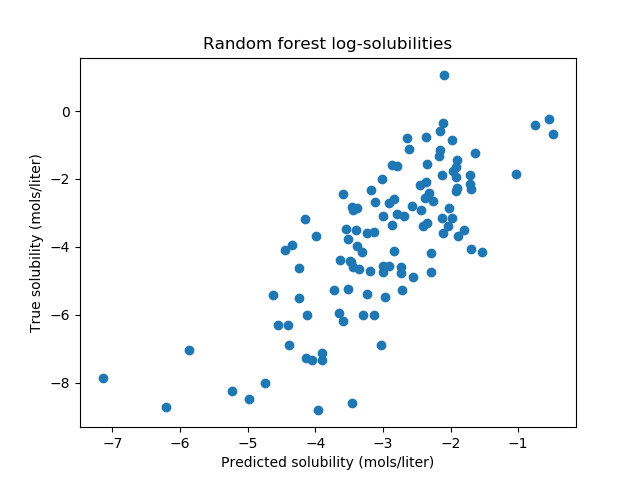
\includegraphics[width=0.5\textwidth]{RFesol}
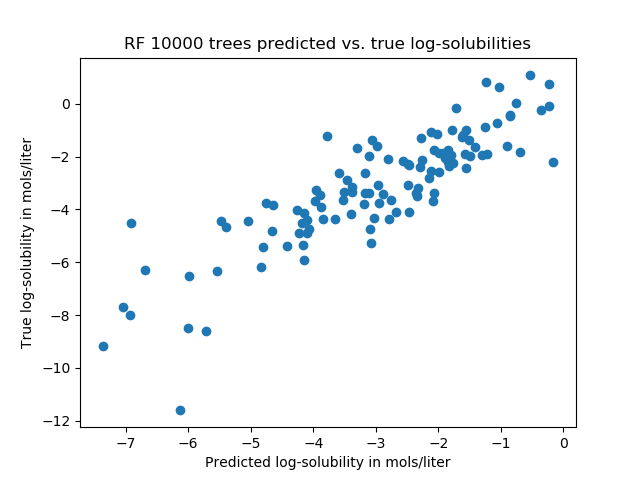
\includegraphics[width=0.5\textwidth]{rfesolrandom10000}

We also used a larger count of estimators (10000) on the CIT Arjuna computing cluster, and obtained a lower RMSE of 2.35. This is shown to the right above.

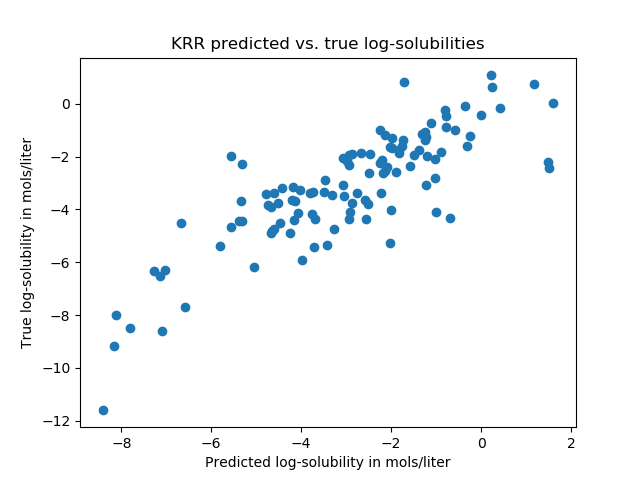
\includegraphics[width=0.5\textwidth]{krr1}

As another conventional model, we trained kernel ridge regression to predict log-solubilities; we used a rbf kernel with hyperparameters taken from the Pande literature. We achieved a remarkable 0.55 RMSE, better than the corresponding Pande benchmark, by using random splits in the data.

\section{Discussion, Timeline, and Division of Work}

As expected, Bemis-Burcko splitting is a stiffer test of the model than random splits. Often, random split data-sets can transfer trained learning on similar compounds over to test time; such circumstances would happen far less often with scaffold splitting.

Given the difference between these initial results and the papers' benchmarks of the same models, there may well be lots of tuning and "fine control" occurring in the Pande results than their discussion would imply. However, these results should be significantly improved upon by the graph representation models to come. We will turn next to these models in our project.

Regarding division of work, Adarsh Dave implemented models for the \texttt{esol} and \texttt{freesolv} datasets. Jake Parker implemented models for the \texttt{qm7} and \texttt{qm7b} datasets. Sarah Malle implemented models for the \texttt{qm8} and \texttt{qm9} datasets.

\section*{References}
\small
[1] Ceder, G.\ \& Persson, K.\ (2013) How Supercomputers Will Yield a Golden Age of Materials Science. {\it Scientific American}, access: \url{https://www.scientificamerican.com/article/how-supercomputers-will-yield-a-golden-age-of-materials-science/}

[2] Wu, Z.\ , Ramsundar, B.\ , Feinberg, E.N.\ , Gomes, J.\ , Geniesse, C.\ , Pappu, A.S.\ , Leswing, K.\ \& Pande, V. (2017) MoleculeNet: a benchmark for molecular machine learning {\it Chem. Sci.}  {\bf 9}(513)

[3] Tetko, I.V.\ , Sushko, Y.\ , Novotarskyi, S.\ , Patiny, L.\ , Kondratov, I.\ , Petrenko, A.E.\ , Charochkina, L.\ , \& Asiri, A.M. (2014) How Accurately Can We Predict the Melting Points of Drug-like
Compounds? {\it J. Chem. Inf. Model.}, 54, 3320--3329

[4] Ramsundar, B, Kearnes, S., Riley, P., Webster, D., Konerding, D. \& Pande, V. (2015) Massively Multitask Networks for Drug Discovery {\it arXiv}, access: \url{https://arxiv.org/pdf/1502.02072.pdf}

[5] Delaney, J. (2004) ESOL: Estimating Aqueous Solubility Directly from Molecular Structure {\it J. Chem. Inf. Model.}

[6] Szisz, D. (2018) Extended Connectivity Fingerprint (ECFP) \url{https://docs.chemaxon.com/display/docs/Extended+Connectivity+Fingerprint+ECFP}

[7] Rupp, M.\ , Tkatchenko, A.\ , Muller, K.R. \ , \& von Lilienfeld, A.O. (2012) Fast and Accurate Modeling of Molecular Atomization Energies with Machine Learning {\it Phys. Rev. Lett.} \textbf{108} 058301

[8] Bemis, G.W., Murcko, M.A. (1996) The Properties of Known Drugs. 1. Molecular Frameworks {\it J. Med. Chem} \textbf{39}(15), 2887–2893
\end{document}